\chapter{Requirements und Use Cases}\label{ch:requirements-und-use-cases}

\section{Systemebene}\label{sec:systemebene}

%% Die Anforderungen aus der Aufgabenstellung sind nicht vollständig. Die Struktur der nachfolgenden Kapitel soll Sie bei der Strukturierung der Analyse unterstützen. Dokumentieren Sie die Ergebnisse der Analysen entsprechend.

\subsection{Stakeholder}\label{subsec:stakeholder}

%% Ermitteln Sie die Stakeholder für das Projekt und listen Sie diese hier auf.

\paragraph{Externe Stakeholder}
\begin{itemize}
    \item Auftraggeber
    \begin{itemize}
        \item Erfüllung aller spezifizierten Anforderungen
        \item Pünktliche Lieferung zum vorgegebenen Termin
        \item Verwendung der vorgegebenen Hard- und Software
    \end{itemize}
    \item Betreuer
    \begin{itemize}
        \item Erreichen der Ziele am Ende jeder Phase
        \item Vollständige Dokumentation als Rückmeldungsgrundlage
    \end{itemize}
    \item Benutzer
    \begin{itemize}
        \item System stellt keine Gefahr dar
        \item Information über Fehlerzustände
        \item Seltenes Eingreifen erforderlich
        \item Hoher \gls{durchsatz}
        \item Einfache Bedienung und Inbetriebnahme (Dokumentation)
    \end{itemize}
    \item Verwaltung TI-Labor
    \begin{itemize}
        \item Keine Beschädigung der \glspl{anlage}
    \end{itemize}
\end{itemize}

\paragraph{Interne Stakeholder}
\begin{itemize}
    \item Entwickler
    \begin{itemize}
        \item Gute Testbarkeit
        \item Einfache Erweiterbarkeit und Modularität
        \item Einheitliche Schnittstellen und Benennungen
        \item Dokumentation (im Code) für Fehlersuche und Teamarbeit
    \end{itemize}
\end{itemize}

\paragraph{Akteure}

\begin{itemize}
    \item \Gls{ctrlp}\\
    Es stellt den \gls{t_start}, \gls{t_stop} und \gls{t_reset} der\gls{anlage} zur Verfügung.

    \item \Gls{belt}\\
    Auf dem \gls{belt} werden \Glspl{workpiece} durch die \Gls{anlage} bewegt.
    \item FTS\_2\\
    Die jeweils andere \gls{anlage} des Systems.
    \item E\_Stop\\
    Ein Button zum Auslösen des Emergency-Stops. Ist er gedrückt, kann er durch Herausziehen
    und drücken des \gls{t_reset} deaktiviert werden.
    \item Metal\_Detector\\
    Sensor zum Erfassen von Metall eines \Gls{workpiece}es.
    \item Height\_Measurement\\
    \gls{lb_he} zum Erfassen der Höhe eines \Gls{workpiece}es.
    \item Stoplight\\
    \gls{ampelled}, die durch verschiedene LED-Einstellungen Zustandsinformationen der \gls{anlage} anzeigt.
    \item Sorting\_Mechanism\\
    Jede \gls{anlage} besitzt einen \Gls{sortierer}.
    Dieser ist in einer von zwei Varianten eingebaut:
    \begin{itemize}
        \item Ejector\\
        Der \gls{ejector}, der bei Stromzufluss ausfährt und so \Glspl{workpiece} in die \gls{rampe} stoßen soll.
        Ohne Strom steht der \gls{ejector} auf \gls{do_not_discard}.
        \item Switch\\
        Die \gls{weiche}, die bei Stromzufluss auf \gls{do_not_discard} steht und \Glspl{workpiece} durchlässt.
        Ohne Strom steht die  \gls{weiche} auf \gls{discard} und befördert \Glspl{workpiece}
        langsam in die \gls{rampe}.
    \end{itemize}
    \item LightBarrier\\
    Das System besitzt diverse Lichtschranken. Sie werden als Trigger und zur Steuerung
    des Kontrollflusses benutzt:
    \begin{itemize}
        \item \gls{lb_st}\\
        Lichtschranke am Anfang eines \gls{belt}es.
        Die Unterbrechung dieser Lichtschranke setzt, vorausgesetzt es liegen keine
        Fehler vor, das \gls{belt} in Bewegung.
        \item \gls{lb_ra}\\
        Lichtschranke an der \gls{rampe}. Aussortierte \Glspl{workpiece} passieren diese Lichtschranke.
        Die Unterbrechung dieser Lichtschranke kann als erfolgreiche Aussortierung interpretiert werden.
        Eine dauerhafte Unterbrechung signalisiert eine volle \gls{rampe}.
        \item \gls{lb_he}\\
        Lichtschranke an der Position des Höhensensors.
        Sie wird als Trigger für den Start der Höhenmessung benutzt.
        \item \gls{lb_sw}\\
        \gls{lb_sw} vor dem \Gls{sortierer} der \gls{anlage}.
        Die Unterbrechung startet die Aussortierung des \gls{workpiece}es, vorrausgesetzt es ist mit \gls{discard} markiert.
        \item \gls{lb_en}\\
        Lichtschranke am Ende eines \gls{belt}es.
        Die Unterbrechung dieser Lichtschranke kann das Transferieren des \Gls{workpiece}es an die nächste \gls{anlage} einleiten.
        Am Ende der zweiten \gls{anlage} werden bei Unterbrechung der \gls{lb_en} \Gls{workpiece}-Informationen an der Konsole ausgegeben.
    \end{itemize}
\end{itemize}

\subsection{Anforderungen}\label{subsec:anforderungen}
%% Welche wesentlichen Anforderungen ergeben sich aus den Systemanforderungen für Ihre Software?
%% Berücksichtigen Sie auch mögliche Fehlbedienungen und Fehlverhalten des Systems.

Im Folgenden werden die Anforderungen an das System definiert. Diese wurden zur besseren
Übersichtlichkeit kategorisiert. Zum besseren Abgleich wird in den
Anforderungen jeweils auf die Sätze in den Anforderungen des Kunden verwiesen, aus denen diese hervorgehen.
Das wird, wie folgendes Beispiel zeigt, gekennzeichnet: (36). 

%! suppress = LabelConvention
\paragraph{\glspl{workpiece} und Sortierung}
\begin{itemize}
    \reqitem{1} Die \gls{anlage} kann zwischen vier Typen von \glspl{workpiece}n unterscheiden (\gls{workpiece_type}) (2, 3, 4, 5, 6)
    \begin{itemize}
        \item \gls{workpiece_flach} (3)
        \item \gls{workpiece_metall} (4)
        \item \gls{workpiece_bohrung} (5)
        \item \gls{workpiece_hoch} (6)
    \end{itemize}
    \reqitem{2} Am Ende des 2.\ \gls{belt}es sollen die \glspl{workpiece} zyklisch in folgender Reihenfolge ankommen (1, 7, 8)
    \begin{enumerate}
        \item \gls{workpiece_metall}
        \item \gls{workpiece_bohrung}
        \item \gls{workpiece_flach}
    \end{enumerate}
    \reqitem{3} \glspl{workpiece}, die nicht in die Sortierreihenfolge passen werden in eine der beiden \glspl{rampe} aussortiert (9, 10)
    \reqitem{4} Der \gls{durchsatz} an \glspl{workpiece} ist zu optimieren (11)
    \reqitem{30} Aussortierung der \glspl{workpiece} soll mit \gls{weiche} funktionieren (41)
    \reqitem{38} Aussortierung der \glspl{workpiece} soll mit \gls{ejector} funktionieren (41)
    \reqitem{39} Beliebige Kombinationen der \gls{sortierer} an den beiden \glspl{anlage} sollen unterstützt werden (42)
    \reqitem{47} Wenn ein \gls{workpiece_bohrung} oder \gls{workpiece_metall} umgedreht wird, ist es ein \gls{workpiece_hoch}
\end{itemize}

\paragraph{Kapazität}
\begin{itemize}
    \reqitem{5} Bei einer vollen \gls{rampe} wird eine Warnung ausgesandt (12)
    \reqitem{6} Wenn die nächste notwendige Aussortierung aufgrund von ausgeschöpfter \glspl{rampe}kapazität
    nicht stattfinden kann, ein Fehler ausgesendet (und somit der Gesamtbetrieb gestoppt) (13)
\end{itemize}

\paragraph{Durchlassablauf}
\begin{itemize}
    \reqitem{7} Zuführung von \glspl{workpiece}n erfolgt durch Einlegen von \glspl{workpiece}n am Anfang von \gls{anlage} 1 (14, 15)
    \begin{itemize}
        \item Ein Unterbrechen der \gls{lb_st} signalisiert dem System das Einlegen eines \gls{workpiece}s,
        sodass der Transport dessen beginnen kann
    \end{itemize}
    \reqitem{9} Das System muss mit in beliebigem Abstand eingelegten \glspl{workpiece}n umgehen können (16, 17) %TODO Mindestabstand
    \begin{itemize}
        \item Solange der Bereich der ersten Lichtschranke frei ist, muss der Benutzer \glspl{workpiece}
        einlegen können, ohne die Korrektheit der Funktion zu gefährden
    \end{itemize}
    \reqitem{14} Der Abstand von \glspl{workpiece}n auf \gls{belt} 2 muss mindestens 25 cm betragen (18)
    \begin{itemize}
        \item Abstand muss vor der Übergabe sichergestellt werden
    \end{itemize}
    \reqitem{16} Auf dem \gls{belt} von \gls{anlage} 2 dürfen sich maximal 2 \glspl{workpiece} befinden (19)
    \reqitem{18} Falls sich bei der Übergabe zwischen den beiden \glspl{belt} ein \glspl{workpiece}
    überschlägt, muss der neue \gls{workpiece_type} beachtet werden (20)
    \begin{itemize}
        \item Der Fall, dass das Teil auf die Seite fällt, sodass es wegrollen könnte, wird ausgeschlossen.
        Wenn sich das \gls{workpiece} überschlägt, ändert sich bei hohen \glspl{workpiece}n der Typ
    \end{itemize}
    \reqitem{20} \glspl{workpiece} dürfen nicht vom \gls{belt} fallen (21)
    \reqitem{24} Beim Einlegen eines \glspl{workpiece}s in die \gls{anlage} soll dem \gls{workpiece} eine eindeutige ID zugewiesen werden(28)
    \reqitem{26} Wenn sich auf einem \gls{belt} kein \gls{workpiece} befindet, stoppt das \gls{belt}
    \reqitem{31} Wenn ein \gls{workpiece} die \gls{lb_en} von FB2 erreicht,
    sollen Informationen zu diesem \gls{workpiece} auf der Konsole ausgegeben werden (22, 23, 24, 25, 26, 27)
    \begin{itemize}
        \item Zu den Informationen zählen die ID, Typ, Höhe auf \gls{anlage} 1 und \gls{anlage} 2 des \gls{workpiece}es als
        auch ein Hinweis darüber, ob sich das \gls{workpiece} überschlagen hat
    \end{itemize}
\end{itemize}

\paragraph{Bedienung durch Taster}
\begin{itemize}
    \reqitem{12} Bei Betätigung von \gls{t_start} wechselt die \gls{anlage} in den Betriebszustand (49)
    \reqitem{15} Bei \gls{longpress} von \gls{t_start} wechselt die \gls{anlage} in den Service-Modus (50)
    \begin{itemize}
        \item Anforderung für den Wechsel ist, dass die \gls{anlage} im Ruhezustand ist
        \item Im Service Modus führt die \gls{anlage} Kalibrierung und Selbsttests durch %TODO Modi in glossar aufnehmen
    \end{itemize}
    \reqitem{17} Bei Betätigung des \gls{t_stop} wechselt die \gls{anlage} in den Ruhezustand (51, 52)
    \begin{itemize}
        \item Wenn Fehler oder Warnung vorliegen, wird stattdessen ein Fehler ausgesandt  %TODO Warnung und Fehler in glossar aufnehmen
    \end{itemize}
    \reqitem{21} Bei Betätigung des \gls{t_reset} werden sämtliche Fehler quittiert (53) %TODO mit kunden kären
    \reqitem{28} Wenn die \gls{anlage} durch \gls{estop} stillgelegt ist, kann der Betrieb durch Drücken des
    \gls{t_reset} der \gls{anlage}, an dem auch der \gls{estop} gedrückt wurde, fortgesetzt werden (56) %TODO 'fortsetzten' mit kunden kären
    \begin{itemize}
        \item Bedingung dafür: Keine \gls{estop} sind gedrückt
    \end{itemize}
    \reqitem{40} Im Service Modus führt die \gls{anlage} Kalibrierung und Selbsttests durch (50) %TODO genauer spezifizieren
    \reqitem{41} Bei Betätigung eines \gls{estop} werden beide \glspl{anlage} angehalten (54, 55)
    \reqitem{42} Dem Benutzer werden Hinweise über die Benutzung der \gls{anlage} mithilfe der LEDs an der \gls{taster}n gegeben
    \begin{itemize}
        \item Im Betriebszustand ist die LED am \gls{t_start} an
        \item Im Ruhezustand die LED am \gls{t_stop}
        \item Bei einem gegangenen oder bestehenden Fehler ist die LED am \gls{t_reset} an
    \end{itemize}
\end{itemize}

\paragraph{Zustandsanzeigen}
\begin{itemize}
    \reqitem{10} Im Betriebszustand leuchtet die grüne \gls{ampelled} dauerhaft (59)
    \reqitem{11} Im Service-Mode blinkt die grüne \gls{ampelled}  (60)
    \reqitem{13} Bei Warnungen blinkt die gelbe \gls{ampelled} (61)
    \begin{itemize}
        \item Eine Warnung ist, dass die \gls{rampe} an der \gls{anlage} voll ist
    \end{itemize}
    \reqitem{19} Wenn im Betriebszustand keine Warnungen vorliegen, ist die gelbe \gls{ampelled} aus (61)
    \reqitem{37} Die rote \gls{ampelled} signalisiert die Fehlerzustände wie folgt (73, 74, 75, 76):
    \begin{itemize}
        \item Anstehend unquittiert wird durch schnelles Blinken (1 Hz) signalisiert (74)
        \item Anstehend quittiert wird durch dauerhaftes Leuchten(75) signalisiert
        \item Gegangen unquittiert wird durch langsames Blinken (0,5 Hz) signalisiert (z.B.\ wenn ein
        \gls{workpiece} an einer \gls{weiche} zu langsam in die \gls{rampe} geschoben wurde) (76)
        \item Steht kein Fehler an, ist die Leuchte aus (73)
    \end{itemize}
    \reqitem{45} Im Ruhezustand leuchtet die \gls{ampel} dauerhaft gelb
\end{itemize}

\paragraph{\gls{weiche}}
\begin{itemize}
    \reqitem{23} Bei Verklemmen der \gls{weiche} wird eine Warnung ausgesandt, bis das \gls{workpiece} in der Rampe ankommt (37)
    \begin{itemize}
        \item Ein \gls{workpiece} ist verklemmt, wenn das \gls{workpiece} länger als erwartet braucht, um in der \gls{rampe} anzukommen
        \item Länger als erwartet wird mit mehr als 50 Prozent der durchschnittlichen Aussortierzeit definiert
    \end{itemize}
    \reqitem{27} Die \gls{weiche} darf nicht länger als 'x' auf offen stehen (35, 36) %TODO 'offen' , zeit festlegen
    \begin{itemize}
        \item Bei minutenlangen Stromfluss wird die \gls{weiche} beschädigt
    \end{itemize}
\end{itemize}

\paragraph{\gls{recorder}}
\begin{itemize}
    \reqitem{25} Es soll eine \gls{record-fn} bereitgestellt werden, mit der ein Benutzer alle
    \glspl{event} der \gls{anlage} in ein \gls{protokoll} aufzeichnen kann (90)
    \reqitem{29} Die von der \gls{record-fn} vorgenommene Aufzeichnung soll menschenlesbar sein (91)
    \reqitem{33} Es soll eine \gls{replay-fn} bereitgestellt werden, mit der ein
    Benutzer eine zuvor aufgezeichnetes \gls{protokoll} abspielen lassen kann (93, 94)
    \reqitem{34} \glspl{protokoll} sollen per Hand angefertigt werden können (95, 96)
\end{itemize}

\paragraph{Höhenmessung}
\begin{itemize}
    \reqitem{32} Bei der Auswertung der Höhenmessung ist die durch Verkippung des Sensors entstehende Abweichung zu berücksichtigen (43, 44)
\end{itemize}

\paragraph{Fehlerumgang}
\begin{itemize}
    \reqitem{35} Nach Behebung eines Fehlers soll der Normalbetrieb fortgesetzt werden (45, 46)
    \begin{itemize}
        \item Nach Möglichkeit sollen die \glspl{belt} nicht geräumt werden
    \end{itemize}
    \reqitem{43} In den Zuständen 'bestehend\_unquittiert' und 'bestehend\_quittiert' bleiben die
    \glspl{belt} beider \glspl{anlage} stehen und der \gls{sortierer} wird der Strom abgestellt
    \begin{itemize}
        \item Die Fehleranzeige mittels der \gls{ampel} ist in\refreq{37}spezifiziert
    \end{itemize}
    \reqitem{36} Fehlerzustand soll wie in Abbildung~\ref{fig:stm-fehlerzustand} beschrieben sein. (65, 66, 67, 69, 70)
    \reqitem{46} Der Fehlerzustand beider \glspl{anlage} wird wie folgt festgelegt:
    \begin{itemize}
        \item Der aktuell bestehende Fehler mit der höchsten Priorität entspricht dem Fehlerzustand der gesamten \gls{anlage}.
        Die Fehlerzustände sind der folgenden Liste nach priorisiert:
    \begin{enumerate} %TODO wording anpassen sodass kein 'priorität' vorkommnt
        \item Anstehend unquittiert
        \item Anstehend quittiert
        \item Gegangen unquittiert
        \item OK
    \end{enumerate}
    \end{itemize}
\end{itemize}

\begin{figure}[h]
    \centering
    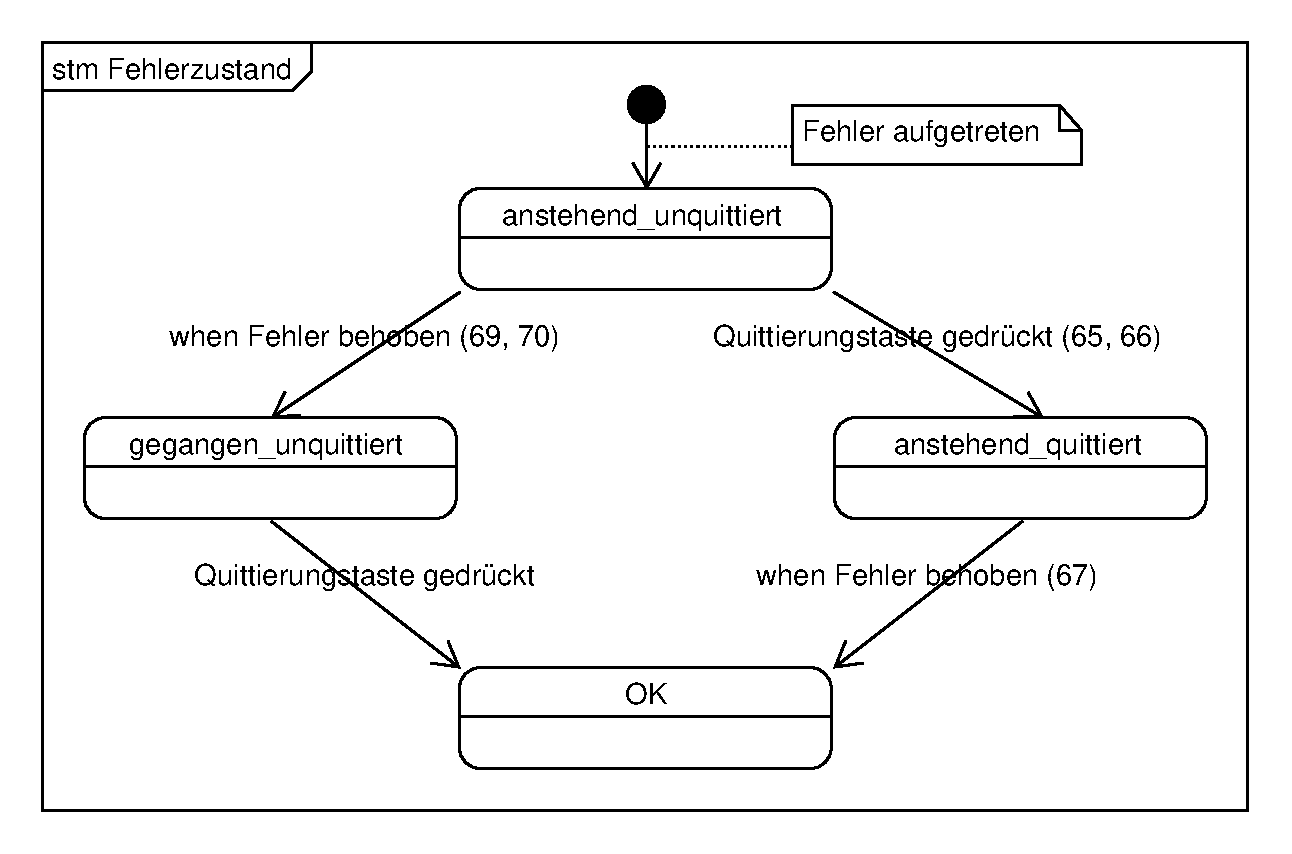
\includegraphics[scale=0.5]{../out/diagrams/stage1/req-fehlerzustand}
    \caption{REQ-36 Visualisierung des Fehlerzustandes eines einzelnen Fehlers}
    \label{fig:stm-fehlerzustand}
\end{figure}

\FloatBarrier

%% In der Aufgabenstellung sind Anforderungen an das System gestellt.
%% Arbeiten Sie diese hier auf und ergänzen Sie diese entsprechend der Absprachen mit dem Betreuer.
%% Achten Sie auf die entsprechende Atribuierung.
%% Berücksichtigen Sie auch mögliche Fehlbedienungen und Fehlverhalten des Systems.

\subsection{Systemkontext}\label{subsec:systemkontext}

%% Wie sieht der Kontext Ihrer Software aus? Wie erfolgt die Kommunikation mit Nachbarsystemen?
%% Liste der ein- und ausgehenden Signale/Nachrichten.


\begin{figure}
    \centering
    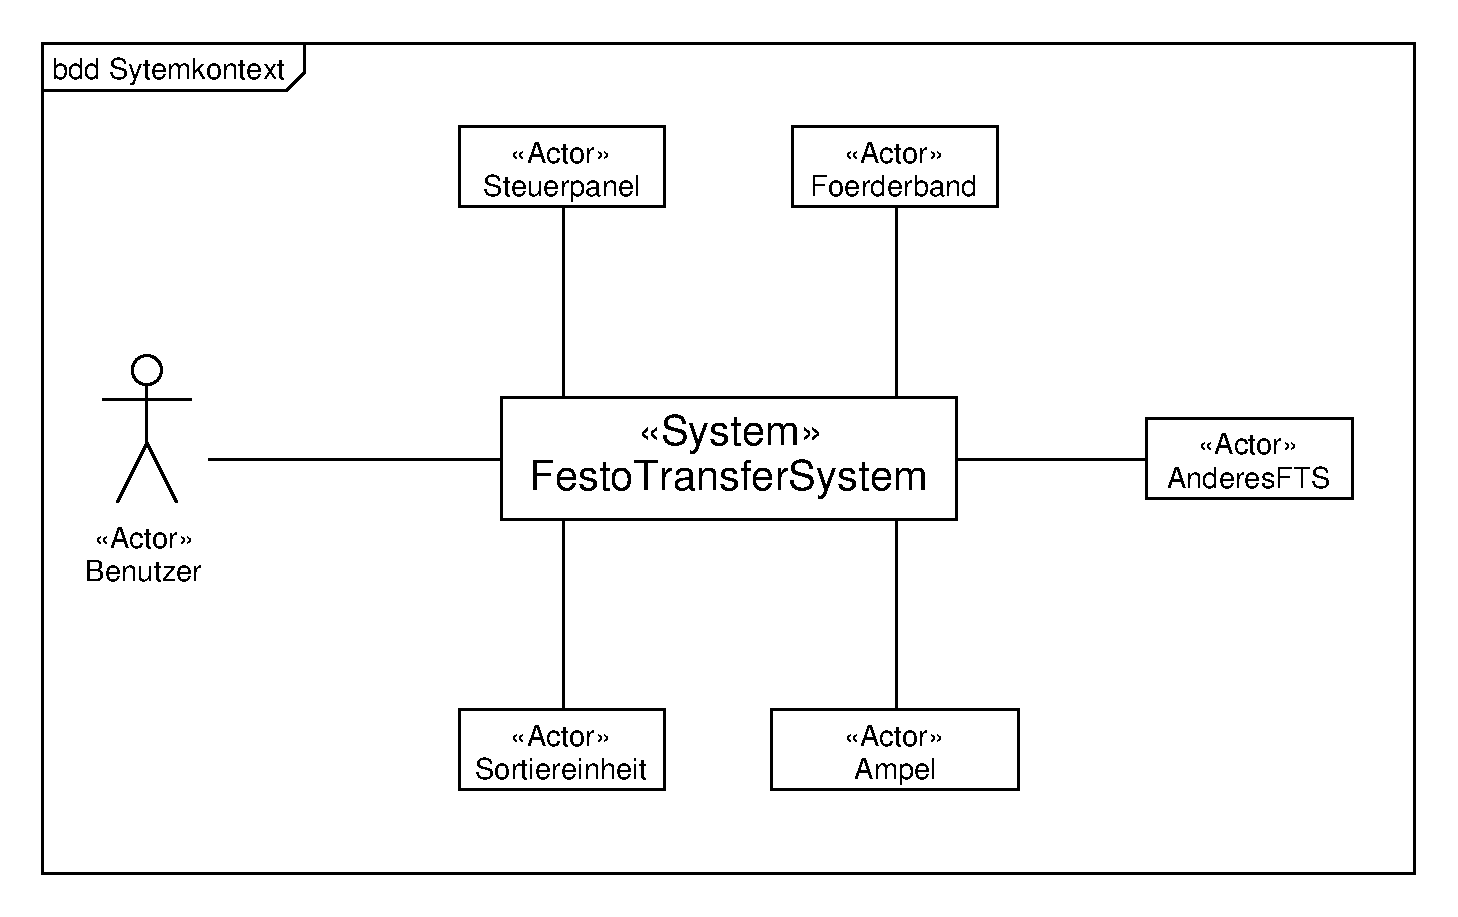
\includegraphics[width=\textwidth]{../out/diagrams/stage1/systemkontext.pdf}
    \caption{Systemkontext}
    \label{fig:systemkontext}
\end{figure}


Betrachte Abbildung~\ref{fig:systemkontext}.
Die Systemsicht bringt umliegende Aktorik des Systemkontext und System selber miteinander in Beziehung.
Die Signalliste ist im Appendix~\ref{ch:signalliste} vorzufinden.

%% Use Cases werden aus einer bestimmten Sicht erstellt.
%% Dokumentieren Sie diese mittels Kontextdiagramm oder Use Case Diagramm.
%% Die Use Cases und Test Cases müssen zu der hier verwendeten Nomenklatur konsistent sein.

\subsection{Use Cases / User Stories}\label{subsec:use-cases-user-stories}

In Abbildung~\ref{fig:ucd} sind die Use Cases in einem Use Case Diagramm dargestellt.
Die Farbgebung dient lediglich zur Veranschaulichung.

\begin{figure}[h]
    \centering
    \makebox[\textwidth][c]{\includegraphics[width=1.2\textwidth]{../out/diagrams/stage1/ucd}}
    \caption{Use Case Diagramm}
    \label{fig:ucd}
\end{figure}

%% Dokumentieren Sie hier, welche Use Cases/ User Stories Sie auf der Systemebene implementieren müssen.
%% Die Test Cases sollen später zu den Use Cases/ User Stories konsistent sein.

%% < Hier kommt die genaue Beschreibung der Use.
%% Pro Anforderung eine Tabelle benutzen. Die Tabelle nach Belieben vervielfältigen. >


\begin{usecase}{01}{\gls{workpiece}-Annahme}{hoch}
    \addTextCollum{Verwandte Requirements}{
        \refreq{7}, \refreq{24}, \refreq{26}
    }
    \addTextCollum{Description}{
        In diesem Use-Case ein \gls{workpiece} von der \gls{anlage} entgegengenommen.
    }
    \addTextCollum{Actors}{
        \gls{belt}, \gls{lb_st}
    }
    \addCollum{Precondition}{
        \item Die \gls{anlage} befindet sich im \gls{betrieb-zst}
        \item Es befindet sich kein \gls{workpiece} im Bereich von \gls{lb_st}
    }
    \addCollum{Trigger}{
        \item \gls{lb_st}
    }
    \addCollum{Main flow}{
        \item[1)] Zuweisung der eindeutigen ID an das betroffene Werkstück
        \item[2)] \gls{belt} ist nicht in Bewegung \textbullet
        \item[3)] \gls{belt} wird in Bewegung gesetzt
        \item[4)] Warte bis \gls{lb_st} nicht mehr unterbrochen \textbullet
    }
    \addCollum{Alternative Flow 1}{
        \item at step 2) of Mainflow
        \item[2a)] \gls{belt} ist bereits in Bewegung und muss nicht gestartet werden
    }
    \addCollum{Alternative Flow 2}{
        \item at step 3) of Mainflow
        \item[3a)] \gls{workpiece} wartet am Ende der Anlage auf Übergabe
    \begin{itemize}
        \item 3a1) \gls{belt} wird nicht gestartet
    \end{itemize}
    }
    \addCollum{Postcondition}{
        \item \gls{workpiece} ist eindeutig erfasst
        \item \gls{lb_st} ist nicht mehr unterbrochen
    }
\end{usecase}


\begin{usecase}{02}{Höhe messen}{hoch}
    \addTextCollum{Verwandte Requirements}{
        \refreq{1}, \refreq{31}, \refreq{32}
    }
    \addTextCollum{Description}{
        Die Höhe eines \gls{workpiece}s wird gemessen.
    }
    \addTextCollum{Actors}{
        Height\_Measurement, LightBarrier\_Height
    }
    \addTextCollum{Preconditions}{
        \item System ist im Betriebszustand
    }
    \addTextCollum{Trigger}{
        LightBarrier\_Height
    }
    \addCollum{Mainflow}{
        \item[1)] Messung bei Height\_Measurement anfragen
        \item[2)] Auf Rückmeldung warten
        \item[3)] Rückgabewert mit den in Höhenprofile erwähnten Werten vergleichen
        \item[4)] Rückgabewert fällt in einen der Bereiche (plus Toleranz) \textbullet
        \item[4)] Jeweiliges Höhenprofil zurückgeben
    }
    \addTextCollum{Postcondition}{
        \item Die Höhe des \gls{workpiece}s ist gemessen
    }
\end{usecase}


\begin{usecase}{03}{Metall erfassen}{hoch}
    \addTextCollum{Verwandte Requirements}{
    \refreq{1}, \refreq{2}, \refreq{3}
    }
    \addTextCollum{Description}{
        In diesem Use-Case wird ein \gls{workpiece_metall} erkannt.
        Initial wird bei jedem \gls{workpiece} von Kunstoff-Material ausgegangen.
    }
    \addTextCollum{Actors}{
        \gls{me_sensor}
    }
    \addCollum{Precondition}{
        \item Das \gls{system} befindet sich im \gls{betrieb-zst}
    }
    \addCollum{Trigger}{
        \item \gls{me_sensor} erfasst Metall
    }
    \addCollum{Mainflow}{
        \item[1)] Aktuellem \gls{workpiece} wird \gls{workpiece_type} \gls{workpiece_metall} zugewiesen
    }
    \addCollum{Postcondition}{
        \item Das Material des \gls{workpiece} ist bekannt.
    }
\end{usecase}

\begin{usecase}{04}{\gls{workpiece} sortieren}{hoch}
    \addTextCollum{Verwandte Requirements}{
        \refreq{1}, \refreq{2}, \refreq{3}, \refreq{6}
    }
    \addTextCollum{Description}{
        Es wird bestimmt, ob ein \gls{workpiece} aussortiert werden soll, oder nicht.
        Dafür muss der Vorgänger \gls{workpiece_type} gespeichert werden.
    }
    \addTextCollum{Actors}{
        Light\_Barrier\_Switch, LightBarrier\_Ramp
    }
    \addTextCollum{Precondition}{
        \item Dem workpiece ist ein \gls{workpiece_type} zugeordnet
    }
    \addTextCollum{Trigger}{
        \item Light\_Barrier\_Switch unterbrochen
    }
    \addCollum{Main flow}{
        \item[1)] Der aktuelle \gls{workpiece_type} wird mit dem erwarteten verglichen
        \item[2)] Das \gls{workpiece} stimmt nicht überein \textbullet
        \item[3)] Das \gls{workpiece} wird aussortiert % TODO UC Referenz
    }
    \addCollum{Alternative flow 1}{
        \item at step 2 of main flow
        \item[2a)] Das \gls{workpiece} stimmt überein
        \begin{itemize}
            \item[2a1)] Das \gls{workpiece} wird durchgelassen % TODO UC Referenz
            \item[2a2)] Ende des use case
        \end{itemize}
    }
    \addCollum{Alternative flow 2}{
        \item at step 3 of main flow
        \item[3a)] Rutsche ist voll und in Primary mode
        \begin{itemize}
            \item[3a1)] das \gls{workpiece} wird durchgelassen
        \end{itemize}
        \item[3b)] Rutsche ist voll und in Secondary mode
        \begin{itemize}
            \item[3b1)] Fehler wird gesendet
        \end{itemize}
    }
    \addTextCollum{Postcondition}{
        \item Das \gls{workpiece} ist sortiert
    }
\end{usecase}


\begin{usecase}{05}{\gls{workpiece} aussortieren}{hoch}
    \addTextCollum{Verwandte Requirements}{
    \refreq{3}, \refreq{5}, \refreq{23}, \refreq{30}, \refreq{38}, \refreq{39}
    }
    \addTextCollum{Description}{
        In diesem Use-Case bewegt der \gls{sortierer} der \gls{anlage} ein \gls{workpiece} vom \gls{belt} in die \gls{rampe}
    }
    \addTextCollum{Actors}{
        \gls{lb_ra}, \gls{sortierer}
    }
    \addCollum{Precondition}{
        \item \gls{system} befindet sich im \gls{betrieb-zst}
    }
    \addCollum{Mainflow}{
        \item[1)] Führe Aussortierung mit \gls{sortierer} durch
        \item[2)] Warte auf Unterbrechung von \gls{lb_ra} \textbullet
        \item[3)] Setze \gls{sortierer} zurück
    }

    \addCollum{Alternative flow 1}{
        \item at step 4) of Mainflow
        \item[4a)] \gls{lb_ra} ist nach zu langer Aussortierzeit nicht unterbrochen worden, \refreq{23}
        \begin{itemize}
            \item[4a1)] Warnung wird gesendet
            \item[4a2)] Warte auf Unterbrechung von \gls{lb_ra}
            \item[4a3)] Sende Nachricht, dass Warnung behoben ist
            \item[4a4)] Go back to step 3) of Mainflow
        \end{itemize}
    }

    \addCollum{Postcondition}{
        \item \gls{workpiece} liegt in der \gls{rampe}
        \item \gls{sortierer} ist zurückgesetzt
    }
\end{usecase}

\begin{usecase}{06}{\gls{workpiece} durchlassen}{hoch}
    \addTextCollum{Verwandte Requirements}{
        \refreq{2}, \refreq{27}
    }
    \addTextCollum{Description}{
        In diesem Use-Case wird ein Werkstück vom Aussortiermechanismus durchgelassen
    }
    \addTextCollum{Actors}{
        Sorting\_Mechanism
    }
    \addCollum{Precondition}{
        \item Die Anlage befindet sich im \gls{betrieb-zst}
    }

    \addCollum{Mainflow}{
        \item[1)] Öffne Sorting\_Mechanism
        \item[2)] Warte bis \gls{workpiece} Sorting\_Mechanism passiert
        \item[3)] Setze Sorting\_Mechanism zurück
    }

    \addCollum{Postcondition}{
        \item Sorting\_Mechanism zurückgesetzt
        \item Werkstück nicht aussortiert
    }
\end{usecase}

\begin{usecase}{07}{\gls{workpiece}-Übergabe}{mittel}
    \addTextCollum{Verwandte Requirements}{
        \refreq{9}, \refreq{14}, \refreq{16}, \refreq{18}, \refreq{31}
    }
    \addTextCollum{Description}{
        In diesem Use-Case erreicht ein Werkstück das Ende des Förderbandes.
        Befindet sich das System in \gls{primary} wird das \gls{workpiece} an die Anlage in \gls{secondary} übergeben.
    }
    \addTextCollum{Actors}{
        Conveyor\_Belt, FTS\_2, LightBarrier\_End
    }

    \addCollum{Precondition}{
        \item Anlage befindet sich im \gls{betrieb-zst}
    }

    \addCollum{Trigger}{
        \item LightBarrier\_End wird unterbrochen
    }

    \addCollum{Mainflow}{
        \item[1)] Die Anlage ist in \gls{primary} \textbullet
        \item[2)] Conveyor\_Belt stoppen
        \item[3)] Anfrage zum transferieren und Werkstück\-Informationen an FTS\_2 senden
        \item[4)] Auf 'OK' von FTS\_2 warten
        \item[5)] Conveyor\_Belt in Bewegung setzen und Werkstück transferieren
    }

    \addCollum{Alternative Flow 1}{
        \item at step 1) of Mainflow
        \item[1a)] Die Anlage ist in \gls{secondary}
        \begin{itemize}
            \item[1a1)] Ausgabe der ID, des Typs, Höhe\_FB1 und Höhe\_FB2 auf der Konsole
            \item[1a2)] Ausgabe an der Konsole, ob sich das Werkstück bei der Übergabe zwischen den Anlagen überschlagen hat
        \end{itemize}
    }

    \addCollum{Postcondition}{
        \item Werkstück ist nicht mehr auf dem Förderband der eigenen Anlage
    }
\end{usecase}

\begin{usecase}{08}{Transfer-Anfrage beantworten}{mittel}
    \addTextCollum{Verwandte Requirements}{
        \refreq{9}, \refreq{14}, \refreq{16}, \refreq{18}, \refreq{31}
    }
    \addTextCollum{Description}{
        In diesem Use-Case geht es um eine Anfrage, ein \gls{workpiece} an diese \gls{anlage} zu übergeben.
        Die Anfrage geht von einer \gls{anlage} in \gls{primary} aus und wird von dieser \gls{anlage}, die sich in \gls{secondary} befindet beantwortet.
    }
    \addTextCollum{Actors}{
        \gls{belt}, \gls{fts2}, \gls{lb_he}, \gls{lb_st}
    }
    \addCollum{Precondition}{
        \item \gls{system} ist im \gls{betrieb-zst}
        \item \gls{anlage} befindet sich im \gls{secondary}
    }
    \addCollum{Trigger}{
        \item Transfer Request mit \gls{workpiece}-Info von \gls{fts2}
    }
    \addCollum{Mainflow}{
        \item[1)] Kein \gls{workpiece} befindet sich zwischen \gls{lb_st} und \gls{lb_he} \textbullet
        \item[2)] Sende 'OK' an \gls{fts2}
        \item[3)] \gls{belt} starten
    }

    \addCollum{Alternative Flow 1}{
        \item at stept 1) of Mainflow
        \item[1a)] Es befindet sich ein \gls{workpiece} zwischen \gls{lb_st} und \gls{lb_he}
        \begin{itemize}
            \item[1a1)] Warten auf Unterbrechung von \gls{lb_he}
            \item[1a1)] Go back to step 2) of Mainflow
        \end{itemize}
    }

    \addCollum{Postcondition}{
        \item Transfer Request beantwortet
    }
\end{usecase}

\begin{usecase}{09}{Durchführung Selbsttests}{mittel}
    \addTextCollum{Verwandte Requirements}{
        \refreq{40}, \refreq{15}, \refreq{11}
    }
    \addTextCollum{Description}{
        Dieser Use-Case beschreibt das Durchführen des \gls{service-mode}.
        Dieser kann durch \gls{longpress} von \gls{t_start} an beiden \glspl{anlage} aktiviert werden.
        Im \gls{service-mode} werden die \glspl{lb_he} kalibriert, die \glspl{belt} getestet sowie
        die korrekte Funktion der
        \gls{sortierer} geprüft. Nach jedem Test muss vom Benutzer am \gls{ctrlp} mit \gls{t_reset}
        das korrekte Verhalten des Systems quittiert werden.
        Die detaillierte Durchführung wird im Kapitel~\ref{subsec:beschreibung-des-servicemode} beschrieben.
    }
\end{usecase}


\begin{usecase}{10}{E-Stop benutzen}{hoch}
    \addTextCollum{Verwandte Requirements}{
        \refreq{41}, \refreq{42}, \refreq{28}, \refreq{44}
    }
    \addTextCollum{Description}{
        Dieser Use-Case beschreibt den Umgang des \gls{system}s bei Betätigung des \gls{estop}.
    }
    \addTextCollum{Actors}{
        \gls{estop}, \gls{fts2}
    }
    \addCollum{Triggers}{
        \item \gls{estop} wird reingedrückt
    }
    \addCollum{Mainflow}{
        \item[1)] Fehlerevent E\_Stop auslösen
        \item[2)] Warten bis \gls{estop} beider \gls{anlage}n rausgezogen
        \item[3)] Fehler behoben senden und quittieren
    }
    \addCollum{Postconditions}{
        \item E-Stop wurde durchgeführt
        \item \gls{system} ist im \gls{ruhe-zst}
    }
\end{usecase}


\begin{usecase}{11}{Wechsel \gls{betrieb-zst}}{hoch}
    \addTextCollum{Verwandte Requirements}{
        \refreq{12}, \refreq{42}
    }
    \addTextCollum{Actors}{
        FTS\_2, Control\_Panel
    }
    \addCollum{Preconditions}{
        \item System ist im \gls{ruhe-zst}
        \item System ist nicht im \gls{fehler-zst}
    }
    \addCollum{Trigger}{
        \item Der Startknopf wird gedrückt
    }
    \addCollum{Mainflow}{
        \item[1)] System wechselt in den \gls{betrieb-zst} \textbullet
        \item[2)] LED im Stopptaster wird eingeschaltet
        \item[3)] LED im Starttaster wird ausgeschaltet \textbullet
    }
    \addCollum{Postconditions}{
        \item[2)] FTS\_2 ist im \gls{betrieb-zst}
        \item[3)] \gls{anlage} ist im \gls{betrieb-zst}
    }
\end{usecase}


\begin{usecase}{12}{Wechsel \gls{ruhe-zst}}{mittel}
    \addTextCollum{Verwandte Requirements}{
        \refreq{17}, \refreq{40}
    }
    \addTextCollum{Description}{
        Dieser Use-Case beschreibt, wie vom \gls{betrieb-zst} in den \gls{ruhe-zst} gewechselt wird.
    }
    \addTextCollum{Actors}{
        \gls{ampel}, \gls{ctrlp}, \gls{fts2}, \gls{belt}, \gls{sortierer}
    }
    \addCollum{Precondition}{
        \item System ist im \gls{betrieb-zst}
    }
    \addCollum{Triggers}{
        \item[1a)] Event Stopptaste empfangen
    }
    \addCollum{Mainflow}
        \item[1)] \gls{belt} abschalten
        \item[2)] \gls{sortierer} zurücksetzen
        \item[3)] \gls{ampelled} wechselt auf gelb leuchtend
        \item[4)] LED am \gls{t_start} vom \gls{ctrlp} einschalten
        \item[5)] LED am \gls{t_stop} vom \gls{ctrlp} ausschalten
        \item[6)] Wechseln in \gls{ruhe-zst}
    }
    \addCollum{Postcondition}{
        \item System ist im \gls{ruhe-zst}
    }
\end{usecase}


\begin{usecase}{13}{Durchführung Selbsttests}{mittel}
    \addTextCollum{Verwandte Requirements}{
        \refreq{40}, \refreq{15}, \refreq{11}
    }
    \addTextCollum{Description}{
        Dieser Usecase beschreibt die Durchführung des Service-Modus 
    }
    \addTextCollum{Actors}{
        \gls{ampel}, \gls{ctrlp}, \gls{fts2}, \gls{belt}, \gls{sortierer}, \gls{t_start}, \gls{t_reset}
    }
    \addCollum{Precondition}{
        \item \gls{system} ist im \gls{ruhe-zst}
    }
    \addCollum{Triggers}{
        \item[1a)] \gls{t_start} \(\geq 3\) sek gedrückt 
    }
    \addCollum{Mainflow}{
        \item[2)] \gls{ampel} auf schnell grün blinken schalten
        \item[3)] \gls{he_sensor} kalibrieren
        \item[4)] \gls{belt} schnell vorwärts für 1 sek
        \item[5)] \gls{belt} schnell Rückwärts für 1 sek
        \item[6)] \gls{belt} stopp
        \item[7)] LED in \gls{t_reset} aktivieren
        \item[8)] Warten auf \gls{t_reset} gedrückt
        \item[9)] LED in \gls{t_reset} deaktivieren] 
        \item[10)] \gls{sortierer} aktivieren
        \item[11)] \gls{sortierer} deaktivieren
        \item[12)] LED in \gls{t_reset} aktivieren
        \item[13)] Warten auf \gls{t_reset} gedrückt
        \item[14)] LED in \gls{t_reset} deaktivieren
        \item[15)] \gls{ampel} auf gelb leuchten schalten
        \item[16)] Wechsel in Ruhezustand
    }
    \addCollum{Postcondition}{
        \item \gls{system} ist im \gls{ruhe-zst}
        \item \gls{he_sensor} ist kalibriert
    }
    \addCollum{Excepional Flow}{
        \item[1)] \gls{t_start} \(\geq 3\) sek gedrückt
        \item[2)] \gls{ampel} auf gelb leuchten schalten
        \item[3)] Wechsel in Ruhezustand
    }
\end{usecase}

\section{Systemanalyse}\label{sec:systemanalyse}

%% Ihr technisches System hat aus Sicht der Software bestimmte Eigenschaften.
%% Was muss man für die Entwicklung der Software in Struktur, Schnittstellen,
%% Verhalten und an Besonderheiten wissen?
%% Wählen Sie eine Kapitelstruktur, die am besten zur Dokumentation Ihrer Ergebnisse geeignet ist.

\subsection{Art des Systems}

Bei dem zu entwerfenden System handelt es sich um die Steuerung eines Festo-Transfersystems,
welche auf dem BeagleBoneBlack Einplatinencomputer, von dem jede \gls{anlage} einen besitzt, zu realisieren ist.
Daher handelt es sich um ein Embedded System.
Für das zu entwickelnde Softwaresystem bedeutet dies, dass es zur Steuerung der Prozesse sehr nah
an der in der \gls{anlage} verbauten Hardware arbeiten muss.
Ein weiterer wichtiger Punkt ist, dass das System mit einer weiteren gleichartigen \gls{anlage} über
das Netzwerk kommunizieren muss. Dies ist ebenfalls im Entwurfsprozess zu berücksichtigen.

\subsubsection{Eigenschaften des BeagleBoneBlack und Grundlagen QNX}

Auf dem BeagleBoneBlack Einplatinencomputer läuft das Echtzeitbetriebssystem QNX, das Kommunikation
zwischen Prozessen und Threads mittels Message Passing bevorzugt.
Dieses Message Passing kann auch über das Netzwerk erfolgen, sodass Messages auch an
einen weiteren BeagleBoneBlack geschickt werden können.
Die Architektur sollte sich daher auf Message-Passing stützen, gerade um die Kommunikation mit der
anderen gleichartigen \gls{anlage} zu erleichtern.
Da der BeagleBoneBlack ein eigenes Stück Hardware mit eigenem Betriebssystem ist, muss für die
Entwicklung die Entwicklungsumgebung QNX Momentics benutzt werden, die Debugging und Testing ermöglicht.
Die Kommunikation mit dem BeagleBoneBlack und dem Entwicklungsrechner erfolgt über die Netzwerkverbindung.

\subsection{Kommunikation mit der Hardware}

Die Ansteuerung der Aktorik und Sensorik der \gls{anlage} erfolgt direkt über die GPIOs des BeagleBoneBlack.
Die Sensorik ist hierbei an GPIO0, die Aktorik des Transfersystems an GPIO1 und die LEDs des \gls{ctrlp}s an GPIO2
gekoppelt.
Bei den GPIOs können Bits einzeln gesetzt und gelöscht werden und es können die aktuellen Werte ausgelesen werden.
Auf Veränderung an den GPIOs kann mittels pro Pin konfigurierbarer Interrupts (steigende Flanke, fallende Flanke,
Level=0, Level=1) reagiert werden.
Interrupts lassen sich nach dem Auslösen für einen einstellbare Zeit ignorieren (Debouncing).
Um später nicht direkt mit den GPIOs interagieren zu müssen, sollte ein Hardware Abstraction Layer
einfachere Schnittstellen zum Ansteuern der Aktorik und für das Reagieren auf die Sensorik bereitstellen.
Der Höhensensor ist am ADC des BeagleBoneBlack angeschlossen. Dieser kann über das Schreiben in ein
bestimmtes GPIO-Register aktiviert werden und kann dann nach erfolgreicher Messung einen Interrupt auslösen.

\subsection{Besonderheiten beim Systemaufbau}

Bei genauerer Betrachtung des Systemaufbaus fallen folgende Eigenschaften und Zusammenhänge besonders auf.
Sie sind bei der Verhaltensmodellierung zu berücksichtigen und könnten das Erkennen von Szenarien vereinfachen.

\subsubsection{Platzierung der \gls{lb_he} bei der Höhenmessung}

Die \gls{lb_he} an der Höhenmessung ist so platziert, dass sich die Mitte eines \Gls{workpiece}es bei ihrer
Unterbrechung genau unter dem Höhenmesser befindet.
Auf diese Art lassen sich die unterschiedlichen Höhen von \Glspl{workpiece}n mittels einer einzelnen Messung unterscheiden.
Die gemessenen Höhen bei unterschiedlichen \glspl{workpiece_type} gehen aus Tabelle~\ref{tab:werkstuecke} hervor.

\begin{table}[h]
    \begin{center}
        \begin{tabular}{ |c|c| }
            \hline
            Form                     & Höhe in mm \\
            \hline\hline
            HOCH                 &  25,0-25,4\\
            \hline
            FLACH                     & 19,8-20,2 \\
            \hline
            LOCH               & 15,8-16,4 \\
            \hline
        \end{tabular}
    \end{center}
    \caption{Höhen der unterschiedlichen \glspl{workpiece_type}}
    \label{tab:werkstuecke}
\end{table}

Ebenso fällt auf, dass der Abstand der \gls{lb_he} für die Höhenmessung vom Anfang des Förderbands ca. 25 cm beträgt,
was für die Bestimmung des Abstands bei der Werkstückübergabe zwischen zwei \glspl{anlage} wichtig ist.

\subsubsection{Der Aufbau im Bereich des \gls{sortierer}s}

Im Transportweg der \Glspl{workpiece} befindet sich an der Stelle, an der ein \Gls{workpiece} vom \gls{sortierer} aussortiert
werden muss, eine Lichtschranke.
Das Unterbrechen dieser Lichtschranke kann daher als Signal zum Starten des Aussortiervorgangs verstanden werden.
Im Falle einer \gls{weiche} als \gls{sortierer} müsste diese auf \gls{do_not_discard} gesetzt werden, falls keine Aussortierung erfolgen soll.
Im Falle eines \Gls{ejector}s müsste dieser auf \gls{discard} gesetzt werden, falls das \Gls{workpiece} aussortiert werden muss.
Oberhalb des \Gls{workpiece}es befindet sich in dieser Position auch der Metallsensor.
Bei einer \gls{anlage} mit \gls{weiche} ist wichtig, dass diese bei längerem Verharren von \gls{do_not_discard} beschädigt werden kann.

\section{Softwareebene}\label{sec:softwareebene}

%% Sie sollen Software für die Steuerung des technischen Systems erstellen.
%% Aus den Anforderungen auf der Systemebene und der Systemanalyse ergeben sich
%% Anforderungen für Ihre Software.
%% Insbesondere wird sich die Software der beiden Anlagenteile in einigen Punkten unterscheiden.
%% Dokumentieren Sie hier die Anforderungen, die sich speziell für die Software ergeben haben.
